\documentclass[border=5pt]{standalone}
\usepackage{fontspec,xeCJK,amsmath,amssymb,tikz,graphicx}\usetikzlibrary{arrows.meta}
\setmainfont{Arial}\setCJKmainfont{PingFang SC}
\definecolor{ink}{HTML}{203340}\definecolor{blue}{HTML}{147E91}\definecolor{pale}{HTML}{EEF6F6}\definecolor{warm}{HTML}{FFF4E5}
\begin{document}\begin{tikzpicture}[x=1cm,y=1cm,every node/.style={text=ink,font=\fontsize{11}{14}\selectfont},box/.style={rounded corners=6pt,draw=blue!25,fill=white},flow/.style={-{Stealth},draw=blue,thick}]
\path[use as bounding box](0,0)rectangle(11,27);\fill[pale](0,0)rectangle(11,27);
\node[font=\fontsize{22}{25}\selectfont\bfseries]at(5.5,26.2){DiT：换掉去噪的主干};
\node[text=blue]at(5.5,25.5){VAE 潜空间 + Transformer + 类别条件};
\draw[box](.3,18.8)rectangle(10.7,25);\node[anchor=west,font=\bfseries\large]at(.6,24.4){A　切块入场｜§3.1--3.2};
\node at(5.5,22.55){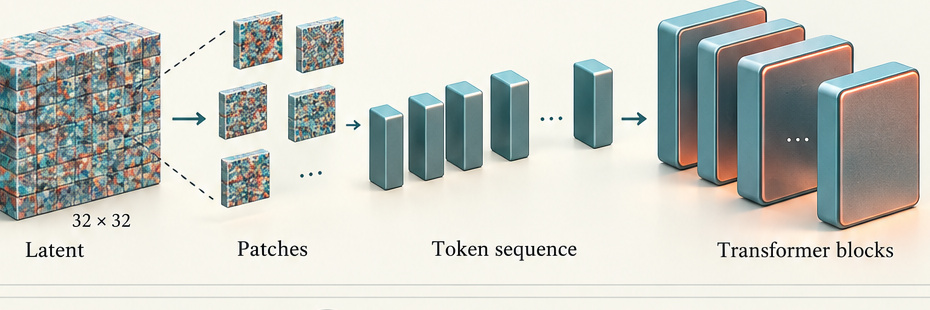
\includegraphics[width=9.5cm]{patch-art.png}};
\node at(5.5,20.7){$256^2\!\times3\xrightarrow{\rm VAE}32^2\!\times4\xrightarrow{+\epsilon}z_t$};
\node at(5.5,20.0){$p=2:\quad256$ 个 patch，$16\to1152$ 维线性投影};
\node at(5.5,19.35){加二维位置编码；输入 $h\in\mathbb R^{256\times1152}$};
\draw[box](.3,10.8)rectangle(10.7,18.4);\node[anchor=west,font=\bfseries\large]at(.6,17.8){B　adaLN-Zero｜§3.2};
\node at(5.5,17.1){$c=e_t+e_y\longrightarrow\gamma_1,\beta_1,g_1,\gamma_2,\beta_2,g_2$};
\node[draw=blue,rounded corners,text width=8.8cm,align=center]at(5.5,15.75){$h\to{\rm LN}\to$ 条件缩放/平移 $\to{\rm MSA}\to\times g_1$};
\node at(5.5,14.9){$u=h+g_1\odot{\rm MSA}((1+\gamma_1)\odot{\rm LN}(h)+\beta_1)$};
\node[draw=blue,rounded corners,text width=8.8cm,align=center]at(5.5,13.75){$u\to{\rm LN}\to$ 条件缩放/平移 $\to{\rm MLP}\to\times g_2$};
\node at(5.5,12.9){$h'=u+g_2\odot{\rm MLP}((1+\gamma_2)\odot{\rm LN}(u)+\beta_2)$};
\node at(5.5,12.0){门初始化为零：$h'=h$；XL 重复 28 个 block};
\node[font=\fontsize{10}{13}\selectfont]at(5.5,11.35){16 个注意力头，各 72 维；调制向量沿 token 维广播};
\draw[box](.3,4.2)rectangle(10.7,10.4);\node[anchor=west,font=\bfseries\large]at(.6,9.8){C　预测、训练与生成｜§3.1--3.2};
\node at(5.5,8.0){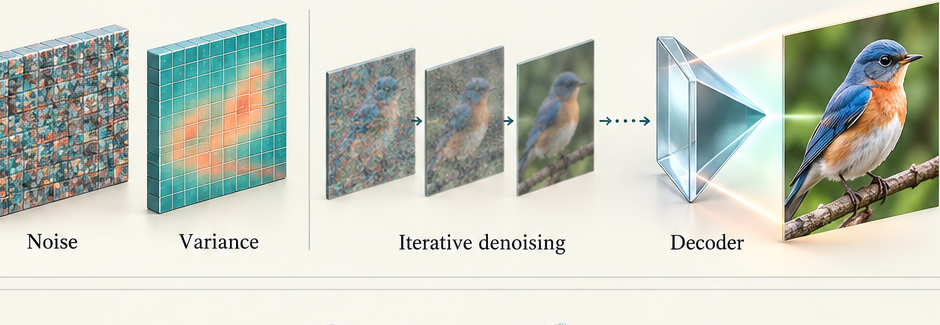
\includegraphics[width=8.0cm]{output-art.png}};
\node at(5.5,6.4){线性输出 + 拼回网格：$32^2\!\times8\to\hat\epsilon,\hat\Sigma$};
\node at(5.5,5.65){训练：噪声 MSE + 方差变分目标；VAE 固定};
\node at(5.5,4.85){生成：高斯噪声，反复 B/C 去噪，最后 VAE 解码};
\draw[box,fill=warm](.3,.3)rectangle(10.7,3.8);\node[anchor=west,font=\bfseries\large]at(.6,3.2){D　扩展实验｜§4--6};
\node at(5.5,2.45){模型深度/宽度、patch 大小、训练量分别改变};
\node at(5.5,1.7){FID、前向计算、训练计算、采样计算分别记账};
\node[font=\fontsize{10}{13}\selectfont]at(5.5,.95){§1--2 提问；§3 A/B/C 拆结构；§4--6 D 核证据};
\end{tikzpicture}\end{document}